This chapter presents an IMP solution which solves issues of OZG identity management described in chapter 3. For utilization of IMP services as described by the IMP solution, an integration architecture is presented which enables the OZG system architecture described in section 2.3 to access the IMP system described in section 2.2.

Focus of the IMP solution and the integration architecture is to require minimal invasion into the existing system architecture: Few existing system components should have to be modified and the existing operation of the system should not be disrupted. The IMP solution should provide an additional but optional way for users to access OZG services.

The integration takes place on three layers:

\begin{center}
    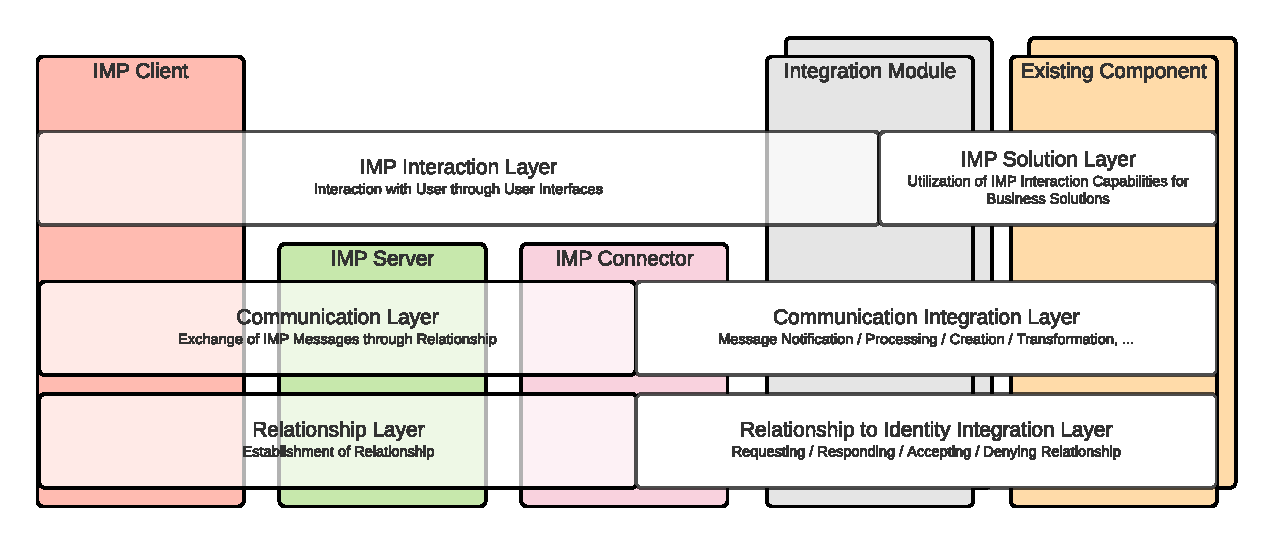
\includegraphics[scale=0.6]{Diagrams/Integration Architecture 1/IMP Layer Diagram Integration.pdf}
\end{center}

\paragraph{IMP Solution Layer} 
The IMP solution is integration on the use case level. It presents possibilities of leveraging interaction capabilities of the IMP system in the context of the service provider for improvement of usability, data protection and security. It describes which types of relationships the service provider can use in his business scenario, how relationships can be processed, which types of messages can be exchanged trough the relationships, what the purpose of each message can be and how the IMP client can react to different message types.

The IMP solution focuses on utilizing IMP capabilities in a way which affects the existing operation of the system architecture the least while solving as many identity management issues described in section 3.1 as possible.

\paragraph{Technological Integration} 
The technological integration is integration on the system level. It consists of an integration architecture enabling the existing systems of the service provider to utilize the IMP system as described by the IMP solution. It is separated into a "Communication Integration Layer" and a "Relationship to Identity Integration Layer". On the "Relationship to Identity Integration Layer" the integration architecture enables the existing systems to create relationship templates and establish relationships. On the "Communication Integration Layer" it enables the existing systems to send and receive different types of IMP messages.

Focus of the technological integration is to connect with as few existing systems as possible while solving as many integration issues described in section 3.3 as possible.

\section{IMP Solution Integration}

\subfile{10-imp_solution_integration}

\section{Technological Integration}

\subfile{11-technological_integration}